\documentclass{article}
\usepackage[utf8]{inputenc}
\usepackage[french]{babel}
\usepackage{amsmath,amssymb}
\usepackage{enumitem}
\usepackage{listings}
\usepackage{color}
\usepackage{graphicx}

\title{TDP n$^o$4\\Multiplication de Fox}
\author{POUSSARD Mark \\ BLAZART Axel}
\date{\today}

\begin{document}
\maketitle

\section{Introduction}
Le but de ce tdp est d'étudier plus en profondeur une méthode transverse de produit de matrice, exploitant cette fois-ci un cluster de calcul. Nous utiliserons donc une approche d'échange de message afin de concevoir notre algorithme et pour l'implémentation nous réaliserons ces échanges grace à la bibliothéque \textbf{MPI}.

\section{Algorithmie de la méthode}
Nous allons à présent décrire le principe et fonctionnement général de la méthode de la multiplication de fox, utilisé ici afin d'effectuer un produit matriciel dans un environnement distribué.
\subsection{Contraintes sur les données acceptés}
Nous nous fixerons cependant des contraintes sur la relation entre le nombre de noeuds de calcul participant à la multiplication et la taille de la matrice à traiter, afin de simplifier l'implémentation de l'algorithme. Nous allons nous concentrer sur des matrices carré distribués toutes de même taille. Cette contrainte implique que le nombre total de processeurs soit capable de diviser la matrice en blocs carrés, et donc que la racine carré du nombre de processeur soit multiple de $n$, la longueur/largeur de nos matrices initiales carrés.\\
Soit $n_{proc}$ le nombre total de processeurs.\\
Soit $n_{mat}$ la taille de notre matrice carré.\\
On doit avoir, $n_{mat} \text{mod} \sqrt{n_{proc}} == 0$
\subsection{Dispersion des données initiales}
Afin de procéder au calcul distribué, il nous faut tout d'abord disperser les données de calcul -c'est à dire les matrices carrés intiales du produit- sur nos noeuds de calcul. On note $m = \frac{n_{mat}}{\sqrt{n_{proc}}}$, et nous considérons alors des quartiers de taille $m \times m$, que nous allons ensuite envoyer sur chaqu'un des noeuds suivant une répartition cartésienne faisant correspondre chaque noeud de calcul à un positionnement dans la matrice global.
\subsection{Echanges et calculs}
Nous allons effectuer $\sqrt{n_{proc}}$ itérations du processus d'envoi/réception des messages et de calcul, afin d'échanger tout les éléments nécessaire à la réalisation de la solution.\\
On note $A$, $B$ et $C$ les matrices de taille $n_{mat} \times n_{mat}$, tel que l'on soit en train de calculer $A \times B = C$\\
Les éléments de la matrice $A$ seront distribué en ligne sur les noeuds de calcul, selon notre communicateur cartésien.\\
Les éléments de la matrice $B$ seront distribué en colonne sur les noeuds de calcul, selon notre communicateur cartésien.\\
A chaque itération, chaque noeud de calcul effectuera son calcul local sur un quartier de la matrice finale $C$.\\
\subsection{Assemblage du résultat}
Le résultat final est ensuite assemblé à partir de chaqu'un des morceaux de matrice distribué sur nos noeuds de calculs. Grace à la distribution cartésienne de nos noeuds de calcul, chaqu'un d'entre eux correspond à un positionnement dans la matrice global qui permet un assemblage de leur résultat local et l'obtention de la matrice $C$ complète.

\section{Résultats}
Nous décrivons maintenant les résultats de l'implémentation qui a été faite de l'algorithme de multiplication de matrice de Fox.

\subsection{Correction}
Afin de vérifier la correction de notre implémentation de l'algorithme, nous implémentons deux cas d'usages sur la base de matrices de tailles données et de contenu soit aléatoir, soit fourni par un fichier de configuration. Dans le cas d'un contenu aléatoire, le résultat est ensuite comparé à un second résultat de multiplication des mêmes matrices, obtenu de manière indépendante.\\
Ces implémentations nous permettent alors de vérifier dans un premier temps de la correction de l'algorithme.
\subsection{Performances}
Nous évaluons ensuite les performances de l'algorithme. Pour ce faire nous comparons les temps d'exécutions entre plusieurs tailles de matrice, et avec plusieurs quantitées de noeuds de calculs (figure \ref{fig:graph_all}).\\

\begin{figure}[h]
\centering
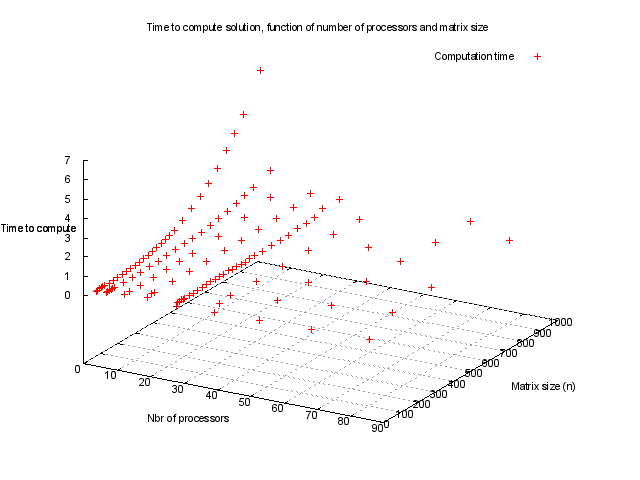
\includegraphics[width=0.6\textwidth]{../perf/results.png}
\caption{Temps d'exécution de l'algorithme selon la taille des matrices d'entrée et du nombre de noeuds de calcul}
\label{fig:graph_all}
\end{figure}

On voit sur le graphe de la figure \ref{fig:graph_all} la tendance du calcul sur de grandes matrices à prendre moins de temps dès que plusieurs noeuds de calcul sont impliqués. La différence est surtout flagrante entre le calcul sur un unique noeud (séquentiel) et le calcul sur 4 noeuds.\\

\begin{figure}[h]
\centering
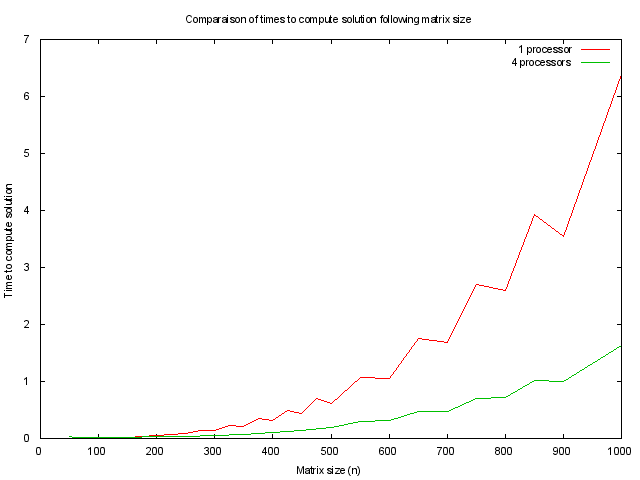
\includegraphics[width=0.6\textwidth]{../perf/results_comp.png}
\caption{Comparaison des temps d'exécution suivant le nombre de noeuds de calculs utilisés}
\label{fig:graph_comp}
\end{figure}

Sur cette figure \ref{fig:graph_comp}, on voit plus précisement les gains de performances que permet l'exécution distribué de l'algorithme.

\begin{figure}[h]
\centering
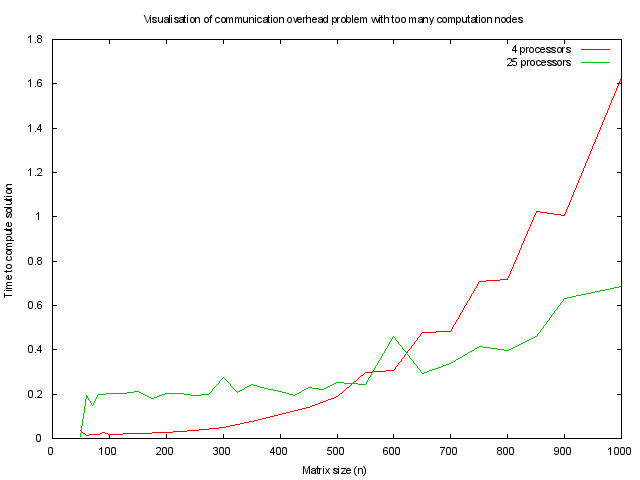
\includegraphics[width=0.6\textwidth]{../perf/results_overhead.png}
\caption{Visualisation de la perte de performances provoquée par un surplus de noeuds de calcul par rapport à la taille du problème}
\label{fig:graph_overhead}
\end{figure}

La figure \ref{fig:graph_overhead} décrit les problèmes qui surviennent lorsque le nombre de noeuds de calcul assigné au problème est trop important par rapport à la taille de ce problème. L'attente et l'envoi de messages afin de procéder à la synchronisation de tout les noeuds de calcul prennent alors trop de temps par rapport avec la quantitée de calcul effectués.

\end{document}
